%% 
%% Copyright 2019-2024 Elsevier Ltd
%% 
%% This file is part of the 'CAS Bundle'.
%% --------------------------------------
%% 
%% It may be distributed under the conditions of the LaTeX Project Public
%% License, either version 1.3c of this license or (at your option) any
%% later version.  The latest version of this license is in
%%    http://www.latex-project.org/lppl.txt
%% and version 1.3c or later is part of all distributions of LaTeX
%% version 1999/12/01 or later.
%% 
%% The list of all files belonging to the 'CAS Bundle' is
%% given in the file `manifest.txt'.
%% 
%% Template article for cas-sc documentclass for 
%% double column output.

\documentclass[a4paper,fleqn]{cas-sc}

% If the frontmatter runs over more than one page
% use the longmktitle option.

%\documentclass[a4paper,fleqn,longmktitle]{cas-sc}

\usepackage[numbers]{natbib}
% \usepackage[authoryear]{natbib}
\usepackage{url}
% \usepackage[authoryear,longnamesfirst]{natbib}
\usepackage{booktabs}
\usepackage{makecell}

%%%Author macros
\def\tsc#1{\csdef{#1}{\textsc{\lowercase{#1}}\xspace}}
\tsc{WGM}
\tsc{QE}
%%%

% Uncomment and use as if needed
%\newtheorem{theorem}{Theorem}
%\newtheorem{lemma}[theorem]{Lemma}
%\newdefinition{rmk}{Remark}
%\newproof{pf}{Proof}
%\newproof{pot}{Proof of Theorem \ref{thm}}

\begin{document}
\let\WriteBookmarks\relax
\def\floatpagepagefraction{1}
\def\textpagefraction{.001}

% Short title
\shorttitle{}    

% Short author
\shortauthors{}  

% Main title of the paper
\title [mode = title]{COVID-19 in Antioquia: A Geospatial Analysis of Case Fatality Rate}  

% Title footnote mark
% eg: \tnotemark[1]
% \tnotemark[1] 

% Title footnote 1.
% eg: \tnotetext[1]{Title footnote text}
% \tnotetext[1]{} 

% First author
%
% Options: Use if required
% eg: \author[1,3]{Author Name}[type=editor,
%       style=chinese,
%       auid=000,
%       bioid=1,
%       prefix=Sir,
%       orcid=0000-0000-0000-0000,
%       facebook=<facebook id>,
%       twitter=<twitter id>,
%       linkedin=<linkedin id>,
%       gplus=<gplus id>]

\author[1]{A. Garcia}%[<options>]

% Corresponding author indication
% \cormark[1]

% Footnote of the first author
% \fnmark[1]

% Email id of the first author
\ead{algarciach@unal.edu.co}

% URL of the first author
% \ead[url]{}

% Credit authorship
% eg: \credit{Conceptualization of this study, Methodology, Software}
% \credit{}

% Address/affiliation
\affiliation[1]{organization={Facultad de Minas, Universidad Nacional de Colombia},
            % addressline={}, 
            city={Medellín},
%          citysep={}, % Uncomment if no comma needed between city and postcode
            % postcode={}, 
            % state={},
            country={Colombia}}

% \author[2]{}%[]

% Footnote of the second author
% \fnmark[2]

% Email id of the second author
% \ead{}

% URL of the second author
% \ead[url]{}

% Credit authorship
% \credit{}

% Address/affiliation
% \affiliation[2]{organization={},
            % addressline={}, 
            % city={},
%          citysep={}, % Uncomment if no comma needed between city and postcode
            % postcode={}, 
            % state={},
            % country={}}

% Corresponding author text
% \cortext[1]{Corresponding author}

% Footnote text
% \fntext[1]{}

% For a title note without a number/mark
%\nonumnote{}

% Here goes the abstract
\begin{abstract}[SUMMARY]
  This study conducted a comparative geospatial analysis of COVID-19 case fatality rates (CFR) across municipalities in Antioquia, Colombia, employing six distinct spatial regression models. We evaluated the performance of Ordinary Least Squares (OLS), Spatial Autoregressive Model (SAR), Spatial Lag Model (SLM), Spatial Error Model (SEM), Geographically Weighted Regression (GWR), and Multiscale Geographically Weighted Regression (MGWR), each designed to address spatial dependence or heterogeneity. OLS, which disregards spatial effects, showed modest explanatory power (Adjusted R$^2$ = 0.2085). SAR and SLM incorporated global spatial autocorrelation through lagged dependent or independent variables, respectively. SEM, by modeling spatial autocorrelation in residuals, achieved the best model fit (AIC = -704.025). GWR, utilizing a fixed Gaussian kernel, allowed for local parameter variations and yielded the highest explanatory power (R$^2$ = 0.560), though with reduced degrees of freedom. In contrast, MGWR, designed for variable-specific bandwidths, exhibited a lower R$^2$ (0.135), suggesting potential underfitting in this specific application. Across all models, altitude and population density consistently emerged as significant predictors of CFR, while humidity and urbanization demonstrated less influence. Spatial models (SLM, SEM, GWR) significantly outperformed OLS, highlighting the critical need to account for spatial dependencies in epidemiological analyses. Among these, SEM offered the optimal balance between parsimony and fit, while GWR underscored the importance of spatial heterogeneity. These findings emphasize the value of spatially explicit modeling in informing public health responses and resource allocation strategies during pandemics.

\end{abstract}


\begin{keywords}
COVID-19\sep Geospatial analysis\sep Spatial regression\sep Antioquia\sep
\end{keywords}

\maketitle

% Main text
\section{Introduction}

The Coronavirus Disease 2019 (COVID-19), caused by the SARS-CoV-2 virus, emerged as a global health crisis following its initial identification in January 2020. On March 11, 2020, the World Health Organization (WHO) officially declared it a pandemic, acknowledging its rapid transmission, high infectivity, and profound global impact on public health, society, and daily life \citep{Franch-Pardo2020,Turbe2020,Cuomo2021}. This unprecedented scenario underscored the urgent need to understand the virus epidemiological and transmission dynamics to inform effective public health interventions and therapeutic strategies.

Understanding the spatiotemporal dynamics of infectious diseases such as COVID-19 is essential for effective mitigation and preparedness. It enables the assessment of outbreak magnitude, guides evidence-based decision-making, and supports targeted public health responses \citep{Franch-Pardo2020}. In this context, Geographic Information Systems (GIS) and spatial analysis have become indispensable tools, allowing researchers to examine disease patterns, identify spatial associations with environmental and socioeconomic variables, and explore transmission mechanisms \citep{Franch-Pardo2020}. Geography, through its integrative and holistic perspective, is particularly well-suited to analyze the complex interactions between biophysical and human factors during a pandemic \citep{Franch-Pardo2020}.

A growing body of research has explored the geographic dimensions of COVID-19, including disease mapping, spatiotemporal modeling, health and social geography, environmental influences, data mining, and interactive web-based visualization \citep{Lin2024}. These studies frequently draw upon large-scale geospatial datasets—commonly referred to as 'big data'—sourced from official COVID-19 dashboards (e.g., Johns Hopkins University, national health ministries), anonymized mobility datasets from technology platforms (e.g., Google, Baidu, Facebook), mobile phone location data, flight itineraries, and social media streams \citep{Franch-Pardo2020,Lin2024}. In addition, environmental (e.g., temperature, humidity) and demographic (e.g., urbanization, population density) variables are often incorporated to enrich the analytical framework \citep{Chen2021,Yu2021,Franch-Pardo2020,Ramrez-Aldana2021,Han2021,Dutta2021,Bherwani2021,Parvin2021,Wheeler2022}.

To examine the relationships between COVID-19 incidence and potential explanatory factors, researchers have employed a range of spatial regression techniques, including Ordinary Least Squares (OLS), the Spatial Lag Model (SLM), and the Spatial Error Model (SEM) \citep{Yu2021,Dutta2021,Aristizabal2024}. More sophisticated approaches such as Geographically Weighted Regression (GWR) and its extension, Multiscale Geographically Weighted Regression (MGWR), have been introduced to account for spatial non-stationarity and heterogeneous relationships across different geographic scales \citep{Han2021,Chen2021,Yu2021,Aristizabal2024}. These models have been instrumental in identifying key predictor variables such as population mobility, socioeconomic disparities (e.g., income, education, access to healthcare), and the role of policy interventions \citep{Ramrez-Aldana2021}.

Among the epidemiological metrics used to assess the severity of the pandemic, the Case Fatality Rate (CFR)—calculated as the ratio of reported deaths to confirmed cases—remains a critical indicator for public health planning and communication with at-risk populations \citep{Das2022,Chaparro2021}. However, accurately estimating CFR is methodologically challenging due to underreporting, delays in case confirmation, and the presence of asymptomatic infections \citep{Paternina-Caicedo2022}.

Addressing the COVID-19 crisis effectively requires an interdisciplinary perspective that integrates data-driven insights, global cooperation, and anticipatory planning \citep{Franch-Pardo2020}. Data visualization and spatiotemporal modeling are vital in uncovering hidden patterns, communicating complex information, and facilitating public engagement \citep{Turbe2020}. Analyzing case data as spatiotemporal phenomena with multi-scale granularity enhances our capacity to implement effective containment and mitigation strategies \citep{AdelaideYeboahForkuo2025,Roy2021,Lin2024}.

This study evaluates spatial patterns and dependencies in Case Fatality Rate (CFR) in confirmed COVID-19 cases across the municipalities of Antioquia, Colombia, using spatial regression models including OLS, SAR, SEM, GWR and MGWR. By doing so, it seeks to contribute to the understanding of spatial health inequalities and to inform targeted public health interventions at the local level.

% \clearpage %%Remove this from your manuscript

\section{Data}

\subsection{Study Area}
The study was conducted in the Department of Antioquia, Colombia, located between 5°30' N and 8°50' N latitude and 73°50' W and 77°00' W longitude. Antioquia encompasses an estimated total area of 62,867 km\textsuperscript{2} and is composed of 125 municipalities, organized into nine subregions. The department has an estimated total population of of approximately 6.903 million for 2024 \cite{DANE_co, DSSA_co}. Figure \ref{DIV-Ant} illustrates the geographical extent and municipal divisions of the study area, along with the spatial distribution of COVID-19 Case Fatality Rate (CFR).

\begin{figure}[htbp]
  \centering
  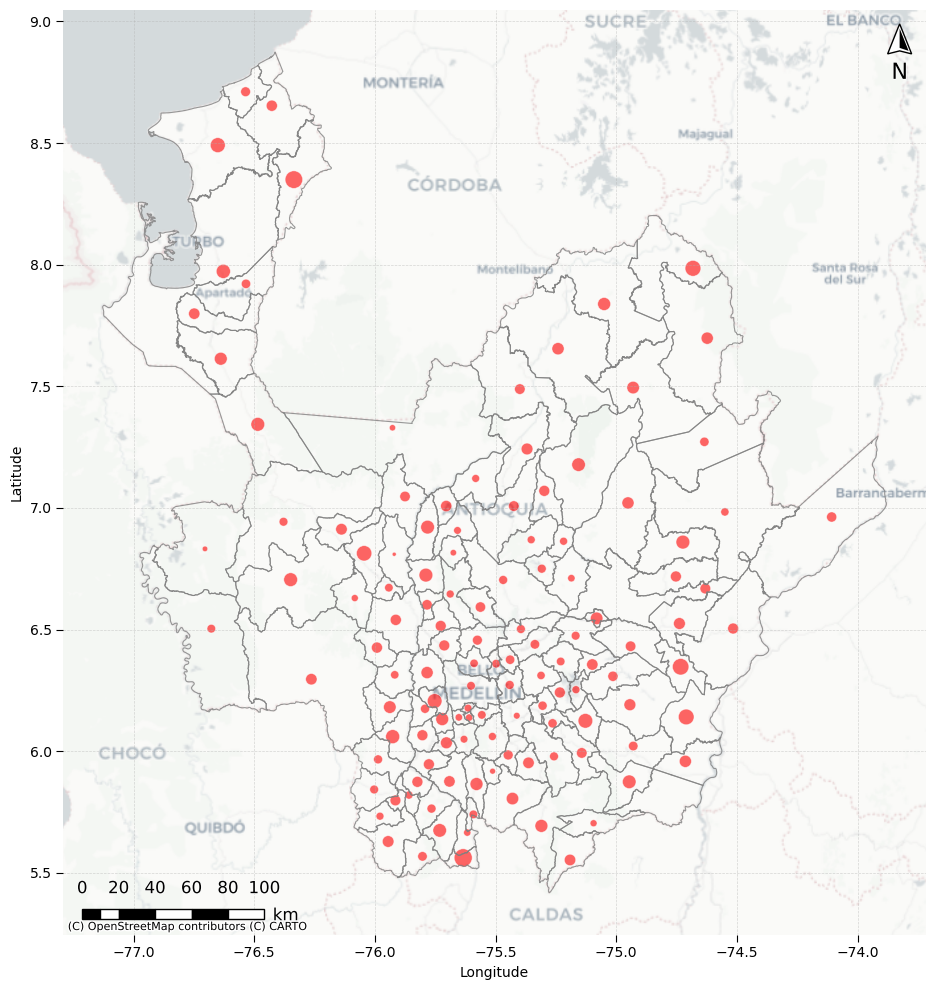
\includegraphics[width=0.8\textwidth]{figures/figure01.png}
  \caption{Map of the study area, the Department of Antioquia, Colombia, showing municipal divisions and spatial distribution of COVID-19 Case Fatality Rate (CFR).}\label{DIV-Ant}
\end{figure}

\subsection{Data Collection}

Demographic and confirmed COVID-19 case data for Colombia were obtained from the Instituto Nacional de Salud (INS) \citep{INS_co} via the national open data portal \citep{DATOS_co}. Population data for the municipalities of Antioquia were sourced from the Departamento Administrativo Nacional de Estadística (DANE) \citep{DANE_co}.

Geographic boundaries and municipal georeferencing information were retrieved from the geoportals of DANE \citep{DANE_co} and the Government of Antioquia \citep{ANT_co}.

Environmental data were also collected. Average municipal altitude was extracted from the NASA Shuttle Radar Topography Mission (SRTM) Digital Elevation Model (30m resolution) \citep{Farr2007}, accessed through Google Earth Engine. Annual mean temperature data were obtained from the WorldClim BIO Variables V1 dataset \citep{Hijmans2005}. Annual mean relative humidity was estimated using the ERA5-Land Monthly reanalysis dataset from the European Centre for Medium-Range Weather Forecasts (ECMWF) \citep{MunozSabater2019}. Both climate datasets were accessed via Google Earth Engine.

The Case Fatality Rate (CFR) \citep{Chaparro2021} was used as the objective variable for this study, serving as a critical indicator to understand the severity and lethality of the virus across different municipalities. The CFR was calculated as the number of known deaths divided by the total number of confirmed cases, expressed as a percentage, following the formula:

$$
\mathit{CFR} = \frac{\mathit{Number\ of\ known\ Deaths\ }}{\mathit{Total\ number\ of\ Confirmed\ cases\ }} \times 100
$$

The initial distribution of the municipal-level (CFR) exhibited strong positive skewness and contained outliers, as shown in Figure \ref{GAUSS-log} (left), rendering it unsuitable for regression models that assume normally distributed residuals. To address this, the response variable was transformed using a logarithmic function $\text{log}(Y + 1)$. This transformation is commonly employed to normalize skewed distributions, reduce the influence of extreme values, and accommodate zero observations \citep{Aristizabal2024}. As a result, the transformed data approximates a continuous distribution with stabilized variance and residuals that more closely follow a Gaussian distribution, as illustrated in Figure \ref{GAUSS-log}, (right).

\begin{figure}
  \centering
  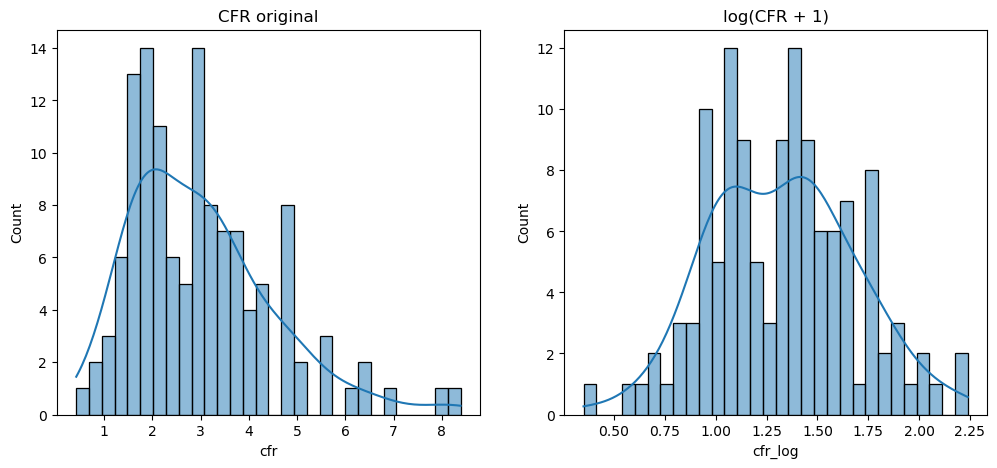
\includegraphics[width=0.8\textwidth]{figures/figure03.png}
  \caption{Distribution of Municipal-Level COVID-19 Case Fatality Rate (CFR) Before and After Logarithmic Transformation.}\label{GAUSS-log}
\end{figure}

The predictive variables considered for this study include: municipal area, total population, population density, annual mean relative humidity, annual mean temperature, and mean altitude. The response variable, a continuous measure, is the Case Fatality Rate (CFR) \citep{Chaparro2021}, serving as an indicator of COVID-19-attributable mortality. The CFR was calculated as the number of known deaths divided by the total number of confirmed cases, expressed as a percentage, following the formula:

The predictive variables in this study included MEAN \citep{Franch-Pardo2020}, mean temperature \citep{Franch-Pardo2020,Ramrez-Aldana2021,Yu2021} and annual mean relative humidity \citep{Franch-Pardo2020,Han2021} as environmental geographic variables, along with urbanization \citep{Dutta2021,Ramrez-Aldana2021} and population density \citep{Franch-Pardo2020,Dutta2021,Bherwani2021,Han2021,Ramrez-Aldana2021,Yu2021,Parvin2021,Yi2021,Putri2023,Wheeler2022} as socioeconomic and demographic indicators. These variables are widely recognized as predictors or influential factors in geospatial analyses of the COVID-19 pandemic

\subsection{Exploratory Spatial Data Analysis}

The spatial distribution of the Case Fatality Rate (CFR) reveals substantial heterogeneity across the region.
To visualize this variation, Figure~\ref{fig:choropleth_cfr} presents a choropleth map of the CFR values.

\begin{figure}[H]
  \centering
  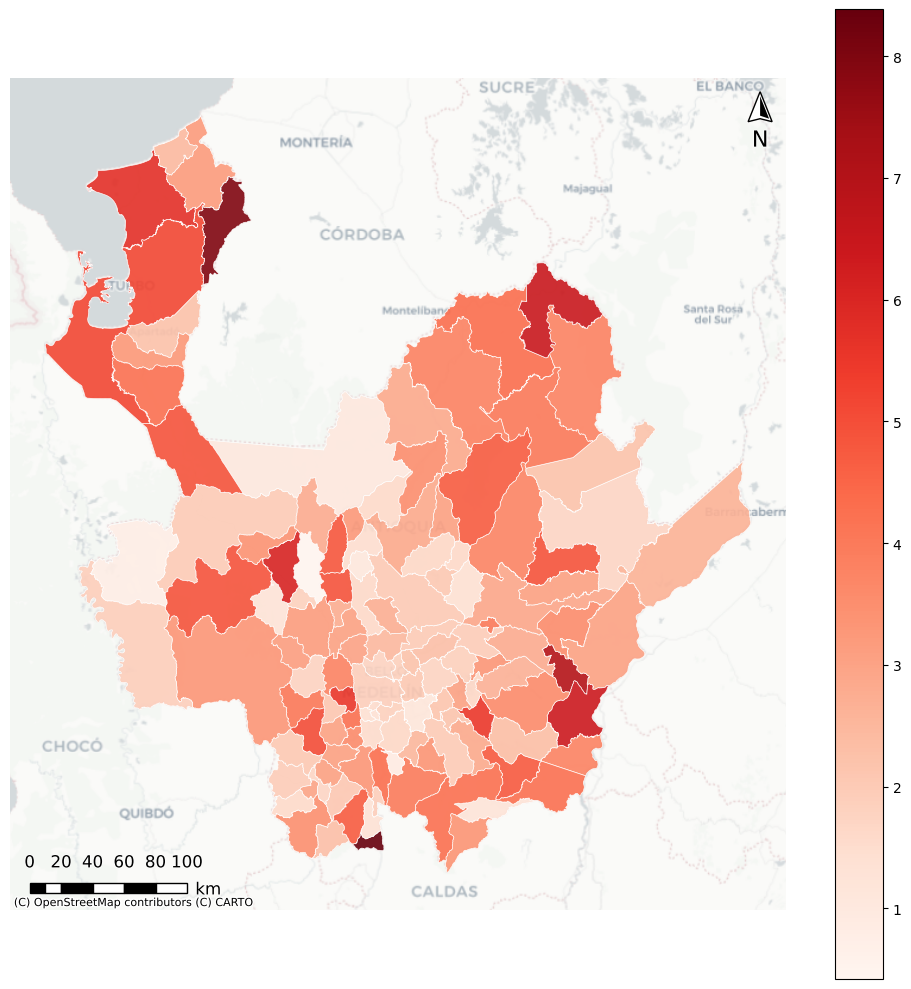
\includegraphics[width=0.75\textwidth]{figures/figure02.png}
  \caption{Spatial distribution of Case Fatality Rate (CFR) COVID-19 cases.}
  \label{fig:choropleth_cfr}
\end{figure}


\subsection{Spatial Regression Models}

\vspace{0.5em}
\subsubsection{Ordinary Least Squares (OLS):}
\begin{equation}
    y = X\beta + \varepsilon,
\end{equation}
where \( y \) is an \( n \times 1 \) vector of observations, \( X \) is an \( n \times k \) matrix of predictors, \( \beta \) is a \( k \times 1 \) vector of coefficients, and \( \varepsilon \sim \mathcal{N}(0, \sigma^2 I) \) are i.i.d. residuals.


\vspace{0.5em}
\subsubsection{Simultaneous Autoregressive Model (SAR)}

The SAR model introduces spatial lag of the dependent variable:

\[
\mathbf{y} = \rho \mathbf{W} \mathbf{y} + \mathbf{X}\boldsymbol{\beta} + \boldsymbol{\varepsilon}
\]

where \( \rho \) is the spatial autoregressive parameter and \( \mathbf{W} \) the spatial weights matrix \citep{Aristizabal2024}.

\vspace{0.5em}
\subsubsection{Spatial Lag Model (SLM)}

The SLM similarly incorporates spatial dependence:

\[
\mathbf{y} = \mathbf{X}\boldsymbol{\beta} + \mathbf{W}\mathbf{X}\mathbf{y} + \boldsymbol{\varepsilon}
\]

with \( \lambda \) representing spatial spillover effects \citep{Aristizabal2024}.

\vspace{0.5em}
\subsubsection{Spatial Error Model (SEM)}

The SEM assumes spatial correlation in the error term:

\[
\mathbf{y} = \mathbf{X}\boldsymbol{\beta} + \lambda\mathbf{W}\mu + \boldsymbol{\varepsilon}
\]

where \( \lambda \) controls residual spatial dependence \citep{Aristizabal2024}.

\vspace{0.5em}
\subsubsection{Geographically Weighted Regression (GWR)}

GWR captures spatial heterogeneity by allowing parameters to vary locally:

\[
y_i = \beta_0(u_i, v_i) + \sum_{k=1}^{p} \beta_k(u_i, v_i)\, x_{ik} + \varepsilon_i
\]

where \( (u_i, v_i) \) are coordinates and \( \beta_k \) are location-specific coefficients \citep{Aristizabal2024}.

\vspace{0.5em}
\subsubsection{Multiscale Geographically Weighted Regression (MGWR)}

MGWR extends GWR by allowing each predictor to operate at a different spatial scale:

\[
y_i = \beta_0(u_i, v_i) + \sum_{k=1}^{p} \beta_k(u_i, v_i; b_k)\, x_{ik} + \varepsilon_i
\]

where \( b_k \) is a variable-specific bandwidth \citep{Aristizabal2024}.

These models were selected to evaluate spatial heterogeneity and autocorrelation effects on CFR variable.

\section{Results}

\subsection{Global Spatial correlation}

The exploratory analysis reveals a non-random distribution of the normalized slope variable, with a positive global Moran's I value of $I = 0.14$, indicating weak but significant spatial autocorrelation (p < 0.05). Figure~\ref{fig:moran}

\begin{figure}[H]
  \centering
  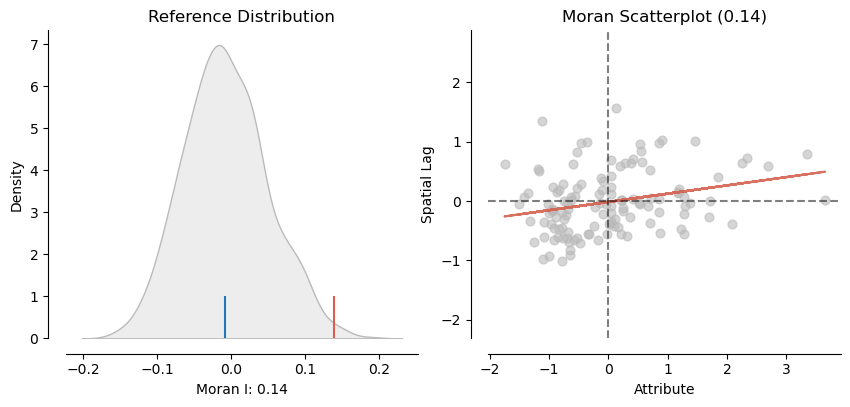
\includegraphics[width=0.8\textwidth]{figures/figure04.png}
  \caption{Reference distribution and Moran's I for the key independent variable}\label{fig:moran}
  \end{figure}

\subsection{Local Spatial Cluster (LISA)}

The Local Indicators of Spatial Association (LISA) analysis reveals significant local clusters in the study area. As illustrated in Figure~\ref{fig:LISA} high-high (HH) clusters, representing municipalities with high slope values surrounded by others with similarly high values, are primarily located in the northern region.  Conversely, low-low (LL) clusters are concentred in the central region.

\begin{figure}[H]
  \centering
  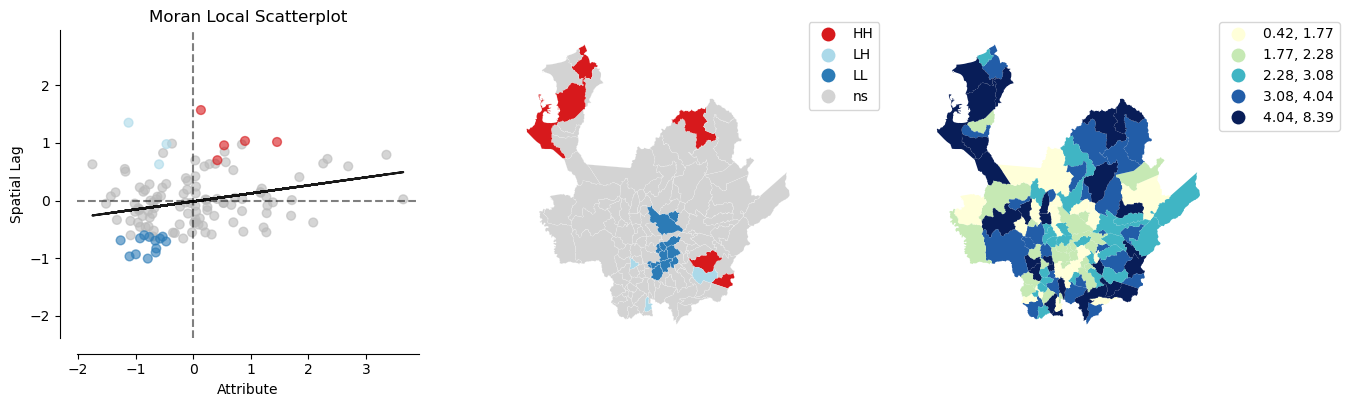
\includegraphics[width=0.8\textwidth]{figures/figure05b.png}
  \caption{LISA Cluster Map of Normalized Slope}\label{fig:LISA}
  \end{figure}

\subsection{Model Comparison}

We evaluated six spatial regression models to analyse the determinants of the COVID-19 case fatality rate (CFR): Ordinary Least Squares (OLS), Spatial Autoregressive Model (SAR), Spatial Lag Model (SLM), Spatial Error Model (SEM), Geographically Weighted Regression (GWR), and Multiscale GWR (MGWR).

As summarized in Table~\ref{tab:spatial_models}, all spatial models outperform the OLS in terms of adjusted R$^2$ or pseudo-R$^2$. Among the global models, the Spatial Error Model (SEM) yields the best overall performance, achieving a relatively high adjusted R$^2$ (0.2458) and the lowest AIC (-699.746). This suggests that spatial autocorrelation in the error terms is a key component in explaining the distribution of CFR.

The SLM and SAR models show comparable R$^2$ values (0.2504 and 0.2458 respectively), but higher AIC values than SEM. While GWR achieves the highest pseudo-R$^2$ (0.560), its AIC (11.443) is substantially worse, indicating potential overfitting or model instability.  MGWR, in contrast, shows the lowest performance in both pseudo-R$^2$ (0.135) and AIC (482.432), suggesting it is not suitable for the dataset.
\begin{table}[htbp]
  \centering
  \caption{Comparative Summary of Regression Models}
  \label{tab:spatial_models}
  \begin{tabular}{@{}lcccccc@{}}
  \toprule
  \textbf{Metric} & \textbf{OLS} & \textbf{SAR} & \textbf{SLM} & \textbf{SEM} & \textbf{GWR} & \textbf{MGWR}\\
  \midrule
  Pseudo-R$^2$/Adjusted R$^2$   & 0.2085   & 0.2458 & 0.2504  & 0.2458  & 0.560 & 0.135 \\
  AIC   & -695.553  & -704.025 & -696.962 & -699.746 & 11.443 & 482.432 \\
  \bottomrule
  \end{tabular}
  \end{table}

  Figure~\ref{fig:sem-residuals} illustrates the spatial distribution of residuals from the Spatial Error Model (SEM). The map shows no clear spatial clustering of residuals, indicating that the SEM effectively accounts for spatial autocorrelation in the data. This absence of systematic patterns in the residuals supports the model's adequacy and confirms the correction of spatial dependence, consistent with its theoretical structure. This visual evidence reinforces the statistical diagnostics, which suggest that the SEM provides the best model fit among those evaluated. 

\begin{figure}[htbp]
  \centering
  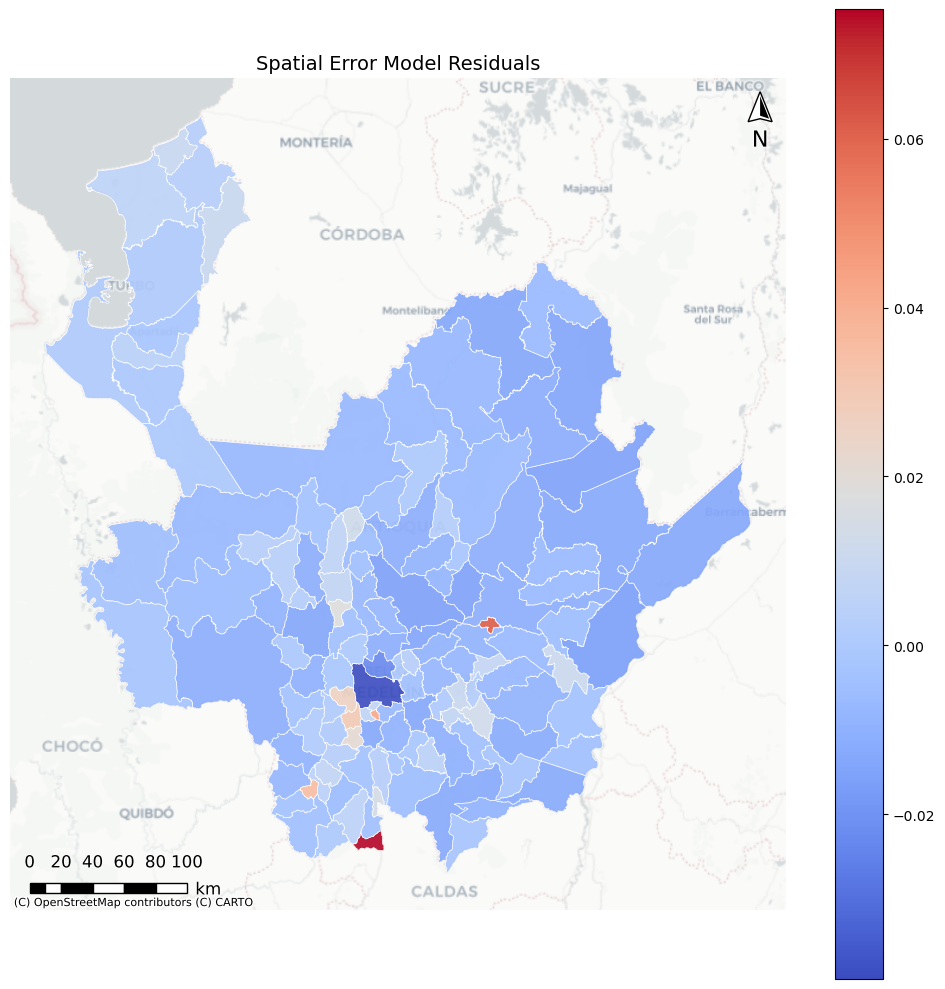
\includegraphics[width=0.8\textwidth]{figures/figure10.png}
  \caption{Spatial distribution of residuals from the Spatial Error Model (SEM). Residual clustering suggests remaining local variation not captured by the global model}\label{fig:sem-residuals}
\end{figure}

\section*{Discussion}

This study analyzed the spatial variation of COVID-19 Case Fatality Rates (CFR) across Antioquia using six regression models: OLS, SAR, SLM, SEM, GWR, and MGWR. Among them, the Spatial Error Model (SEM) showed the best performance, with the lowest AIC (-704.025) and a good pseudo R$^2$ (0.2458), indicating that spatial correlation in the residuals is important and must be considered.

Although the GWR model achieved a higher pseudo R$^2$ (0.560), its high AIC (11.443) suggests overfitting, likely due to its complexity and limited sample size. MGWR performed worse, possibly because the multiscale structure was not strong in this dataset.

Altitude and population density were the most consistent and significant predictors of CFR. In contrast, variables like humidity and urbanization were not statistically significant. This may be due to the lack of health system variables, such as hospital capacity or ICU availability.

High CFRs in small municipalities may reflect few deaths over low case counts (e.g., 3 deaths out of 30 cases = 10\%). Such instability affects model robustness. Future models should include healthcare access, comorbidities, and age structure to improve explanatory power.


% To print the credit authorship contribution details
\printcredits

%% Loading bibliography style file
\bibliographystyle{model1-num-names}
% \bibliographystyle{cas-model2-names}

% Loading bibliography database
\bibliography{covid19-refs}

\end{document}

